% Esquema de la arquitectura del modelo (marco teorico).
% Fuente de images/esquema_modelo.pdf. Para regenerarlo:
%   cd images; pdflatex esquema_modelo.tex
\documentclass[11pt,tikz,border=1pt]{standalone}
\usepackage[T1]{fontenc}
\usepackage[utf8]{inputenc}
\usepackage{lmodern}
\usepackage[sc]{mathpazo}
\usetikzlibrary{positioning,arrows.meta,calc}
 
\definecolor{azul}{HTML}{1F5FA8}
\definecolor{verde}{HTML}{2E9A5E}
\definecolor{tinta}{HTML}{2B2B2B}
\definecolor{suave}{HTML}{5E5E5E}
 
\newcommand{\tit}[1]{\textbf{#1}}
\newcommand{\sub}[1]{{\scriptsize\color{suave}#1}}
 
\begin{document}
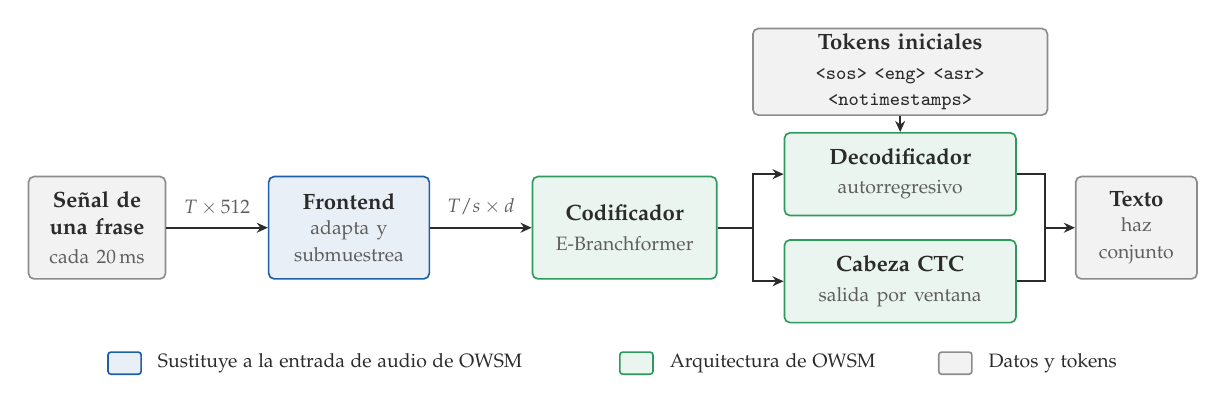
\begin{tikzpicture}[
    font=\footnotesize, text=tinta,
    >={Stealth[length=4pt,width=3.6pt]},
    flecha/.style={->, draw=tinta, line width=0.6pt},
    linea/.style={draw=tinta, line width=0.6pt},
    caja/.style={draw, rounded corners=2pt, line width=0.6pt, align=center,
                 minimum height=1.30cm, inner sep=2pt},
    datos/.style={caja, draw=black!45, fill=black!5},
    nuevo/.style={caja, draw=azul, fill=azul!10},
    owsm/.style={caja, draw=verde, fill=verde!10},
    cabeza/.style={owsm, minimum height=1.05cm},
    forma/.style={font=\scriptsize, text=suave},
  ]
 
  % ---------------------------------------------------------------- modelo
  \node[datos, text width=1.60cm] (senal) at (0.85,0)
    {\tit{Señal de\\una frase}\\[1pt]\sub{cada 20\,ms}};
  \node[nuevo, text width=1.90cm] (front) at (4.05,0)
    {\tit{Frontend}\\[1pt]\sub{adapta y\\submuestrea}};
  \node[owsm, text width=2.20cm] (cod) at (7.55,0)
    {\tit{Codificador}\\[1pt]\sub{E-Branchformer}};
  \node[owsm, cabeza, text width=2.80cm] (dec) at (11.05,0.68)
    {\tit{Decodificador}\\[1pt]\sub{autorregresivo}};
  \node[owsm, cabeza, text width=2.80cm] (ctc) at (11.05,-0.68)
    {\tit{Cabeza CTC}\\[1pt]\sub{salida por ventana}};
  \node[datos, text width=1.40cm] (texto) at (14.05,0)
    {\tit{Texto}\\[1pt]\sub{haz\\conjunto}};
  \node[datos, minimum height=0.85cm, text width=3.6cm] (prompt) at (11.05,1.98)
    {\tit{Tokens iniciales}\\[1pt]{\scriptsize\ttfamily <sos> <eng> <asr> <notimestamps>}};
 
  % flechas, con la forma de la secuencia encima
  \draw[flecha] (senal) -- node[forma, above=1pt] {$T \times 512$} (front);
  \draw[flecha] (front) -- node[forma, above=1pt] {$T/s \times d$} (cod);
  \coordinate (rama) at ($(cod.east)+(0.45,0)$);
  \draw[linea] (cod.east) -- (rama);
  \draw[flecha] (rama) |- (dec.west);
  \draw[flecha] (rama) |- (ctc.west);
  \draw[flecha] (prompt) -- (dec);
  \coordinate (junta) at ($(texto.west)+(-0.38,0)$);
  \draw[linea] (dec.east) -| (junta);
  \draw[linea] (ctc.east) -| (junta);
  \draw[flecha] (junta) -- (texto.west);
 
  % ---------------------------------------------------------------- leyenda
  \begin{scope}[shift={(1.20,-1.72)}, font=\scriptsize]
    \tikzset{muestra/.style={rounded corners=1pt, minimum width=0.42cm,
                              minimum height=0.28cm, line width=0.6pt}}
    \node[muestra, draw=azul, fill=azul!10] at (0,0) {};
    \node[anchor=west] at (0.30,0) {Sustituye a la entrada de audio de OWSM};
    \node[muestra, draw=verde, fill=verde!10] at (6.50,0) {};
    \node[anchor=west] at (6.80,0) {Arquitectura de OWSM};
    \node[muestra, draw=black!45, fill=black!5] at (10.55,0) {};
    \node[anchor=west] at (10.85,0) {Datos y tokens};
  \end{scope}
\end{tikzpicture}
\end{document}
